\input{Dissertation/appendixsetup}   % Предварительные настройки для правильного подключения Приложений
\chapter{Описание микросфер и сорбента на его основе, участвующих в эксперименте} \label{AppendixA}

\section{Микросферы МС-В-1Л}


\begin{figure}[h!]
\centering
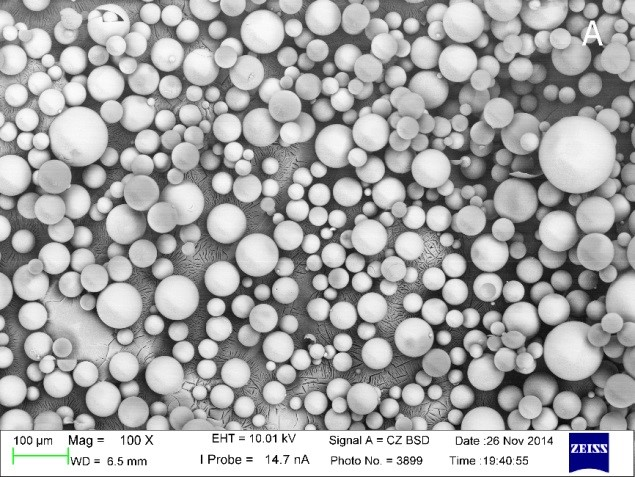
\includegraphics[width=0.8\textwidth]{appendix/MS-V-1L_small} \\
\medskip
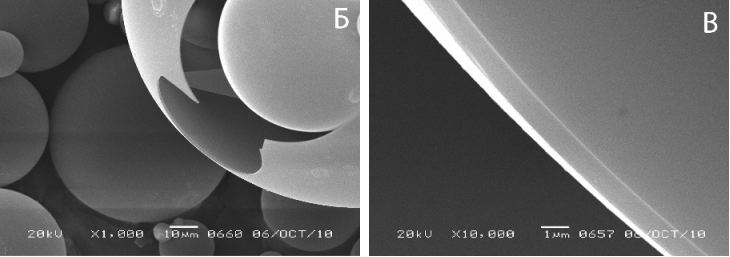
\includegraphics[width=0.8\textwidth]{appendix/MS-V-1L_big}
\caption{Фотографии микросфер МС-В-1Л, сделанные с помощью электронного микроскопа}
\label{pic:MS-V-1L}  
\end{figure}
\begin{figure}[h!]
	\centering
	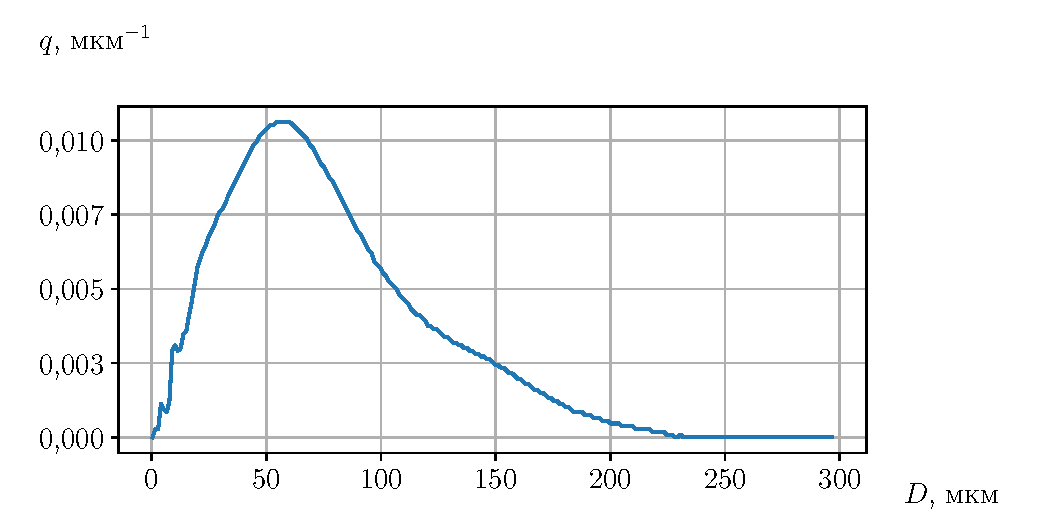
\includegraphics[width=0.95\linewidth]{appendix/MS-V-1L_distr.pdf}
	\caption{Распределение микросфер МС-В-1Л по размерам, полученное методом лазерной дифракции }
	\label{pic:MS-V-1L_distr}  
\end{figure}

\newpage
\begin{longtable}{|p{5cm}|c|}
	\caption{Основные свойства микросфер МС-В-1Л по данным производителя}\label{tbl:MS-V-1L}\\
	[-0.45\onelineskip]
	\hline
	\multicolumn{2}{|c|}{Состав} \\
	\hline
	SiO$_2$ &  76-78~\% \\
	\hline
	Na$_2$O & 11-13~\%\\
	\hline
	CaO & 4-5~\%\\
	\hline
	B$_2$O$_3$ & 4-5~\% \\
	\hline
	ZnO$_2$ & 1-2~\% \\
	\hline
	насыпная плотность	& 0,18-0,22~г/см$^3$ \\
	\hline
	диаметр микросфер	& 10-90~мкм\\
	\hline
	толщина стенок &	$\approx$1~мкм\\
	\hline
\end{longtable}

\newpage
\section{Микросферы МС-ВП-А9}

Синтетические микросферы МС-ВП-А9 пятой группы, аппретированные $\gamma$-минопропил-триэтоксиланом. Микросферы МС-ВП-А9, обладают наивысшей гидростатической прочностью, значение давления, при котором происходит разрушение 10~\% частиц, для исследуемого образца составляет 177~кгс/см$^2$ (10~\% уровень разрушения частиц в воде, методика НПК «Терм» ТУ 6-48-91-92), насыпная плотность 0,383 г/см$^3$. Микросферы имеют сферическую форму и однородную-гладкую поверхность и внешне схожи с микросферами МС-В-1Л.

\begin{figure}[h!]
	\centering
	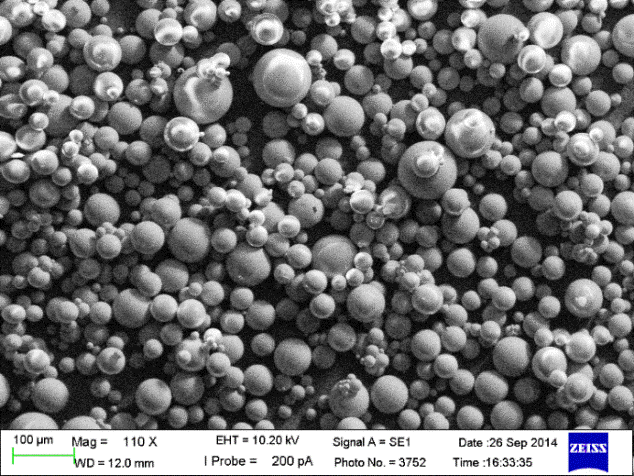
\includegraphics[width=0.6\textwidth]{appendix/MS-VP-A9_1} \\
	\medskip
	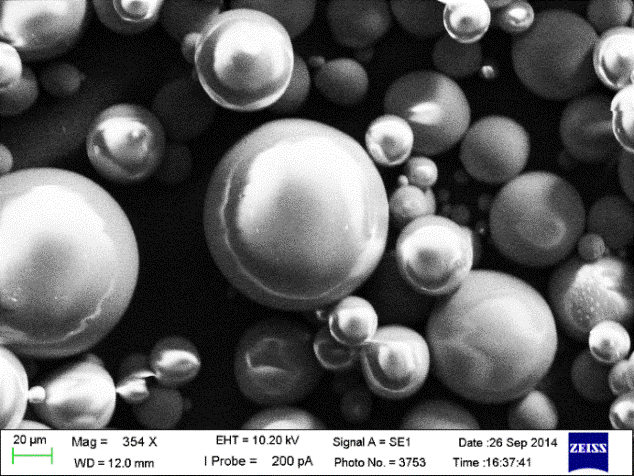
\includegraphics[width=0.6\textwidth]{appendix/MS-VP-A9_2}
	\caption{Фотографии микросфер МС-ВП-А9, сделанные с помощью электронного микроскопа}
	\label{pic:MS-VP-A9}  
\end{figure}


\newpage
\section{Кремнеземные микросферы}

Отличительной особенностью данного типа микросфер является их химический состав, содержание SiO$_2$ больше $80$~\% и малое количество примесей. Насыпная плотность образца $0,2$~г/м$^3$, размер частиц варьируется в диапазоне от $12$ до $240$~мкм, средний диаметр равен $52$~мкм. Частицы так же имеют гладкую однородную поверхность. 

\begin{figure}[h!]
	\centering
	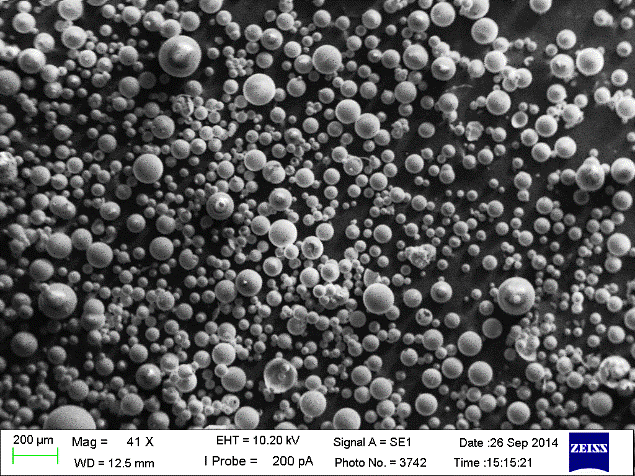
\includegraphics[width=0.65\textwidth]{appendix/SiO2_micr_1} \\
	\medskip
	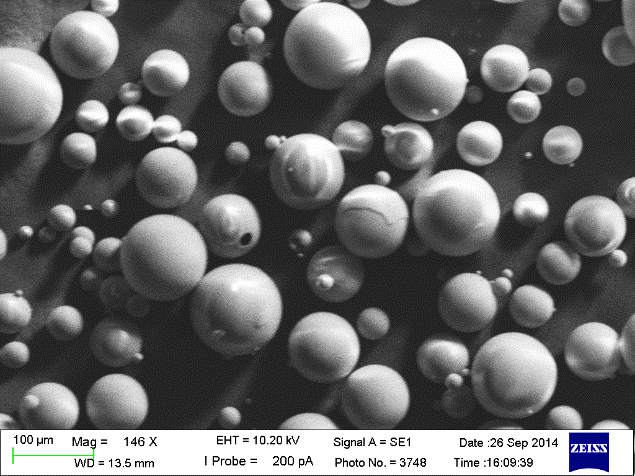
\includegraphics[width=0.65\textwidth]{appendix/SiO2_micr_2}
	\caption{Фотографии кремнеземных микросфер, сделанные с помощью электронного микроскопа}
	\label{pic:SiO2_micr}  
\end{figure}


\newpage
\section{Ценосферы  НМ-R-5А -0,16 мм (vv vac)}

Образцы исходных ценосфер НМ-R-5А -0,16 мм (vv vac), характеризующиеся ограничением по диаметру сверху (до $160$~мкм) и средней толщиной стенки 8 мкм, насыпная плотность образца $0,43$~г/м$^3$. Размер частиц варьируется в пределах от $35$ до $155$~мкм, со средним значением в районе $70$~мкм. По химическому составу выделенные ценосферы представляют собой многокомпонентные системы SiO$_2$-Al$_2$O$_3$-Fe$_2$O$_3$-CaO-MgO-Na$_2$O-K$_2$O-P$_2$O$_5$-MnO с содержанием стеклофазы и фазы муллита в районе $62,8$ и $35,5$ мас.~\% соответственно и Al$_2$O$_3$~$39$~мас.~\%. 
По данным электронной микроскопии образец ценосфер содержит как гладкие сферические частицы, так и большое количество частиц с пористой оболочкой неправильной формы. Ценосферы предоставлены ИХХТ СО РАН, г. Красноярск.

\begin{figure}[h!]
	\centering
	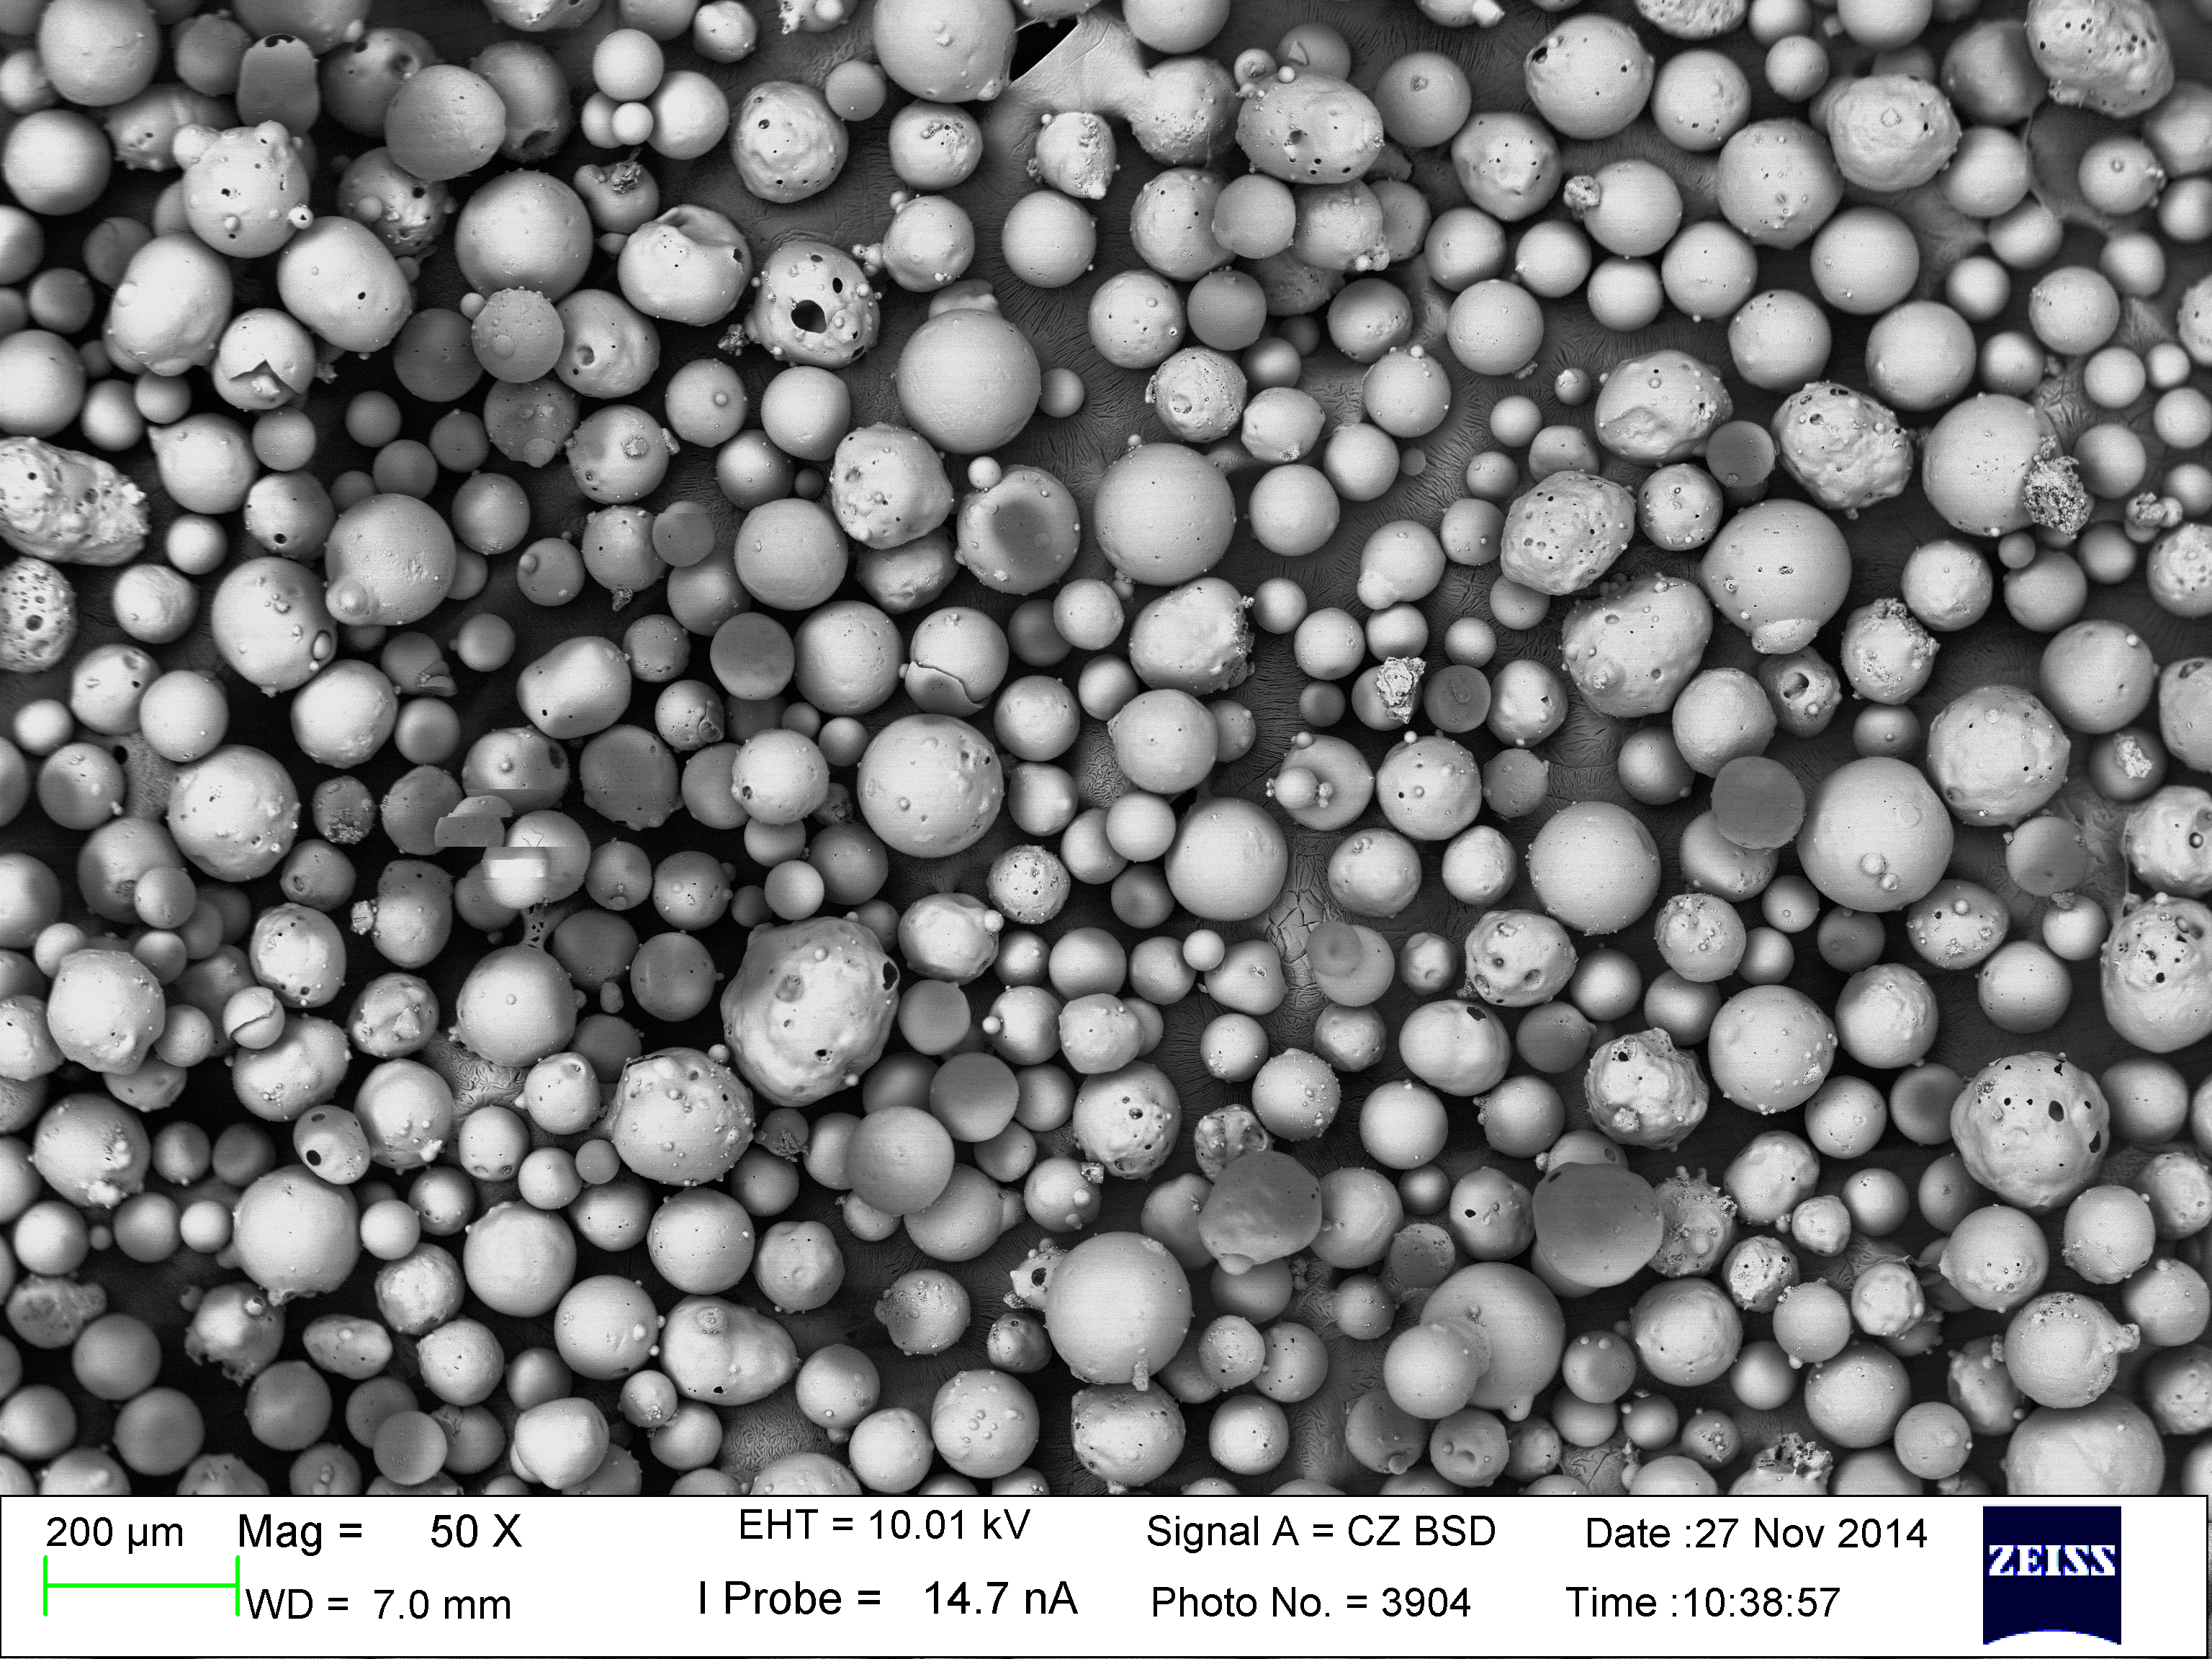
\includegraphics[width=0.49\textwidth]{appendix/HMR-5A_1}~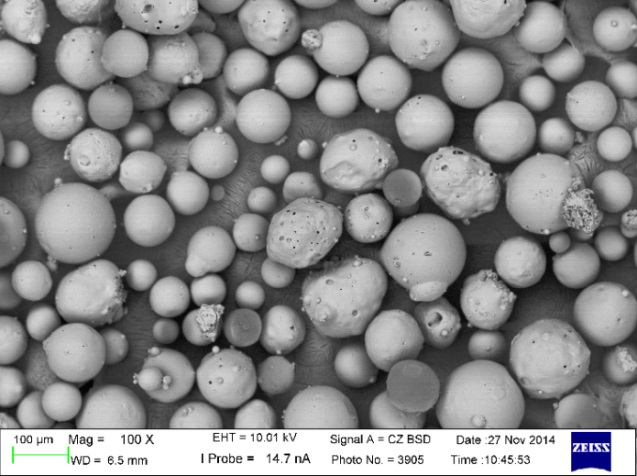
\includegraphics[width=0.49\textwidth]{appendix/HMR-5A_2}
	\caption{Фотографии ценосфер  НМ-R-5А -0,16 мм (vv vac), сделанные с помощью электронного микроскопа}
	\label{pic:HM-R-5A}  
\end{figure}

\newpage
\begin{figure}[h!]
	\centering
	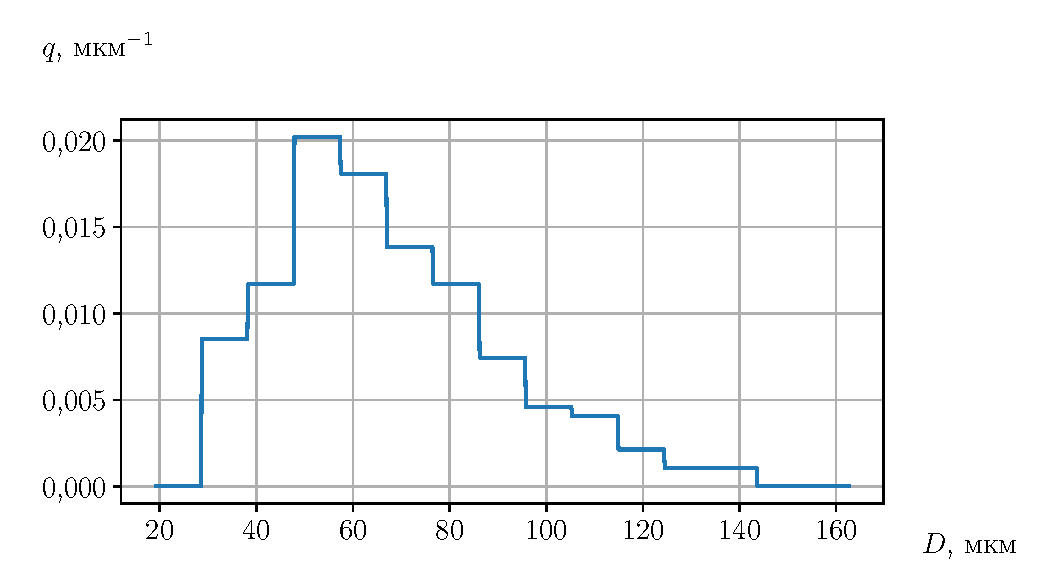
\includegraphics[width=0.9\linewidth]{appendix/HMR-5A_distr}
	\caption{Распределение ценосфер НМ-R-5А -0,16 мм (vv vac) по размерам, полученное на основе анализа фотографий образцов}
	\label{pic:HM-R-5A_distr}  
\end{figure}





\newpage
\section{Ценосферы НМ-R-5А 0.063+0.05 мм 1000~\textcelsius}

С целью получения сорбента с увеличенной гелиевой проницаемостью, исходные ценосферы НМ-R-5А проходили дополнительную сортировку и обработку, включающую раскристаллизацию оболочки частиц. Фракция неперфорированных ценосфер меньшего размера НМ-R-5А 0.063+0.05~мм (частицы просеивались через систему сит с размером ячейки $63$ и $50$~мкм, средний диаметр частиц $57$~мкм, толщина оболочки $3$ мкм), насыпная плотность образца $0,41$~г/м$^3$ подвергалась дополнительной термообработке при $1000$~\textcelsius. При этом в оболочке частиц образуется дополнительная фаза муллита, отличающаяся от исходной меньшим размером кристаллов, что может приводить к увеличению гелиевой проницаемости стеклокристаллической оболочки по границам раздела фаз <<муллит – стекло>>.  Ценосферы предоставлены ИХХТ СО РАН, г. Красноярск.


\begin{figure}[h!]
	\centering
	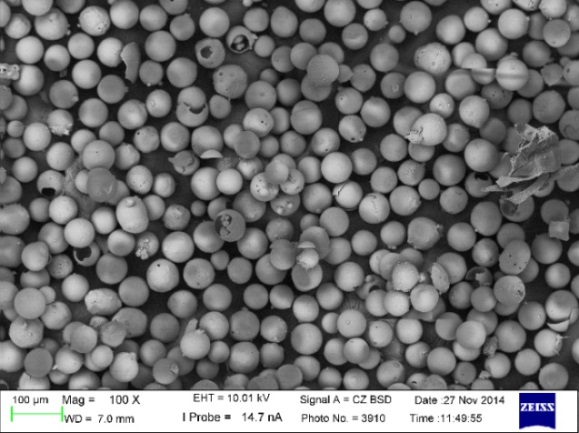
\includegraphics[width=0.49\textwidth]{appendix/HMR-5A_1000_1}~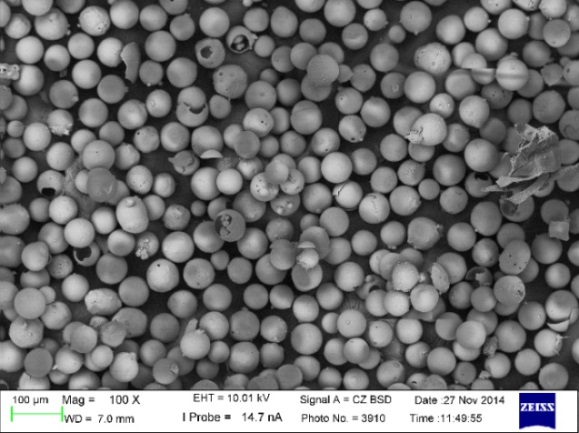
\includegraphics[width=0.49\textwidth]{appendix/HMR-5A_1000_1}
	\caption{Фотографии ценосфер  НМ-R-5А 0.063+0.05 мм 1000~\textcelsius, сделанные с помощью электронного микроскопа}
	\label{pic:HMR-5A_1000_1}  
\end{figure}

\newpage
\section{Композитный сорбент на основе микросфер МС-В-1Л}

В качестве гелий проницаемого компонента композитного сорбента для процесса выделения гелия, использовались синтетические стеклянные микросферы МС-В-1Л, связующим материалом служил – гидроксид алюминия (псевдобемит). Сорбент изготовлен в ИППУ СО РАН, г. Омск.

\begin{figure}[h!]
	\centering
	\fbox{	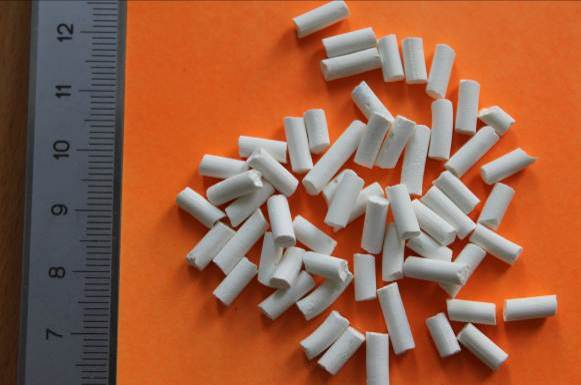
\includegraphics[width=0.95\textwidth]{appendix/comp_sorb_MS-V-1L} }
	\caption{Фотография композитного сорбента	ПБ-15~\%МС  на основе микросфер МС-В-1Л}
	\label{pic:comp_sorb_MS-V-1L}  
\end{figure}


\begin{longtable}{|l|p{2cm}|p{2cm}|p{2cm}|p{2cm}|p{2cm}|}
	\caption{Основные характеристики композитного сорбента на основе микросфер МС-В-1Л}\label{tbl:comp_sorb_MS-V-1L}\\
[-0.45\onelineskip]	
	\hline
	&
	$S_{\text{уд}}$, м$^2$/г & 
	$V_{\text{пор}}$, см$^3$/г & 
	Проч\-ность, кг/см$^2$ & 
	Насып\-ная плотность, г/см$^3$ &
	Объем сорб. пр-ства, см$^3$/г \\
	\hline
	ПБ-15~\%МС &
	$160$ &
	$0,46$ &
	$33,2$ & 
	$0,41$ & 
	не менее $0,4$\\
	\hline
\end{longtable}

